\documentclass[a4paper,11pt]{article}

\usepackage[utf8]{inputenc}

\usepackage{graphicx}
\usepackage{caption}
\usepackage{subcaption}

\usepackage{pgfplots}
\pgfplotsset{compat=1.18} 

\usepackage{minted}

\begin{document}

\title{
    \textbf{REPORT NAME}
}
\author{Edward Sharp}
\date{06-02-25}

\maketitle

\section*{Introduction}

\section*{Selection Sort}

The selection sort algorithm is done by having an inner loop and an outer loop.
The outer loop divides the array into two subarrays, one is sorted (beginning on the left),
and the other is unsorted (the remaining elements).
In each iteration of the outer loop \texttt{(i)}, the algorithm processes the \texttt{(i)}-th position.
It then selects the smallest element from the unsorted part of the array and places it in the \texttt{(i)}-th position.

\begin{minted}{c}
for (int i = 0; i < n -1; i++)
  {
    ...
  }
\end{minted}

A variable \texttt{(candidate)} is then used to track the index of the smallest element in the unsorted array,
this is assumed to be at position \texttt{i} initially.

Then there is the inner loop which iterates over all the remaining elements in the unsorted subarray (from \texttt{j = i + 1} to \texttt{j = n}).
For each element, it checks if the current element \texttt{(arr[j])} is smaller than the current smallest candidate \texttt{(arr[candidate])}.

\begin{minted}{c}
for (int j = i + 1; j < n ; j++)
{
  if (arr[j] < arr[candidate])
  {
    candidate = j;
  }
}
\end{minted}

After exiting the inner loop, the smallest element in the unsorted subarray has been determined,
and its index is stored in \texttt{candidate}.
This element \texttt{(arr[candidate])} is swapped with the current position \texttt{(arr[i])} of the unsorted subarray.

\begin{minted}{c}
int temp = arr[i];
arr[i] = arr[candidate];
arr[candidate] = temp;
\end{minted}

\begin{figure}[h!]
  \centering
  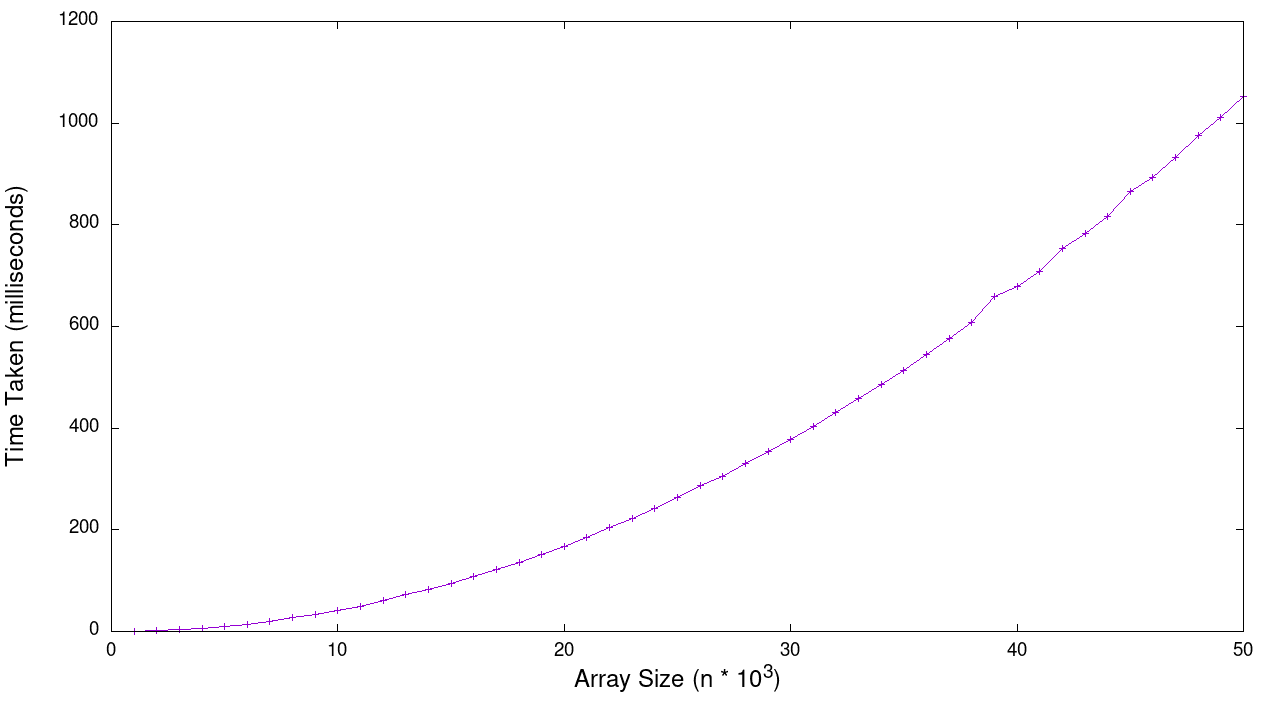
\includegraphics[width=0.8\textwidth]{SelectionSort_plot}
  \caption{Selection sort, array size plotted against time}
  \label{fig:SelectionSort_plot}
\end{figure}

Even if the array is already sorted, the algorithm will still compare all elements to find the smallest candidate.
The outer loop runs $(n - 1)$ iterations in total, and for each iteration, the inner loop scans the unsorted subarray,
running $(n - i - 1)$ times.
This gives us a time complexity of $O(n^2)$.
This time complexity can be observed in figure 1, where we see the start of the positive side of a parabola from our plotted results.

\section*{Insertion Sort}
With insertion sort, the goal is to insert the current element into its correct position within the sorted portion of the array,
as the algorithm processes each element.
The outer loop is the same as for the one used in selection sort.
For each iteration of the outer loop, the inner loop is used to move the current element backwards through the sorted portion of the array,
(from \texttt{j = i} to \texttt{j > 0}), until it is in the correct position.
At each step, any elements larger than the current element are swapped with the current element.

\begin{minted}{java}
for (int j = i; j > 0 && arr[j] < arr[j - 1]; j--)
{
  swap(&arr[j], &arr[j - 1]);
}
\end{minted}

This is done with the \texttt{swap} function:

\begin{minted}{java}
void swap(int *a, int *b)
{
    int temp = *a;
    *a = *b;
    *b = temp;
}
\end{minted}

At the end of each iteration of the outer loop, the current element is inserted into the sorted portion of the array,
and the size of the sorted subarray grows by 1.

\begin{figure}[h!]
  \centering
  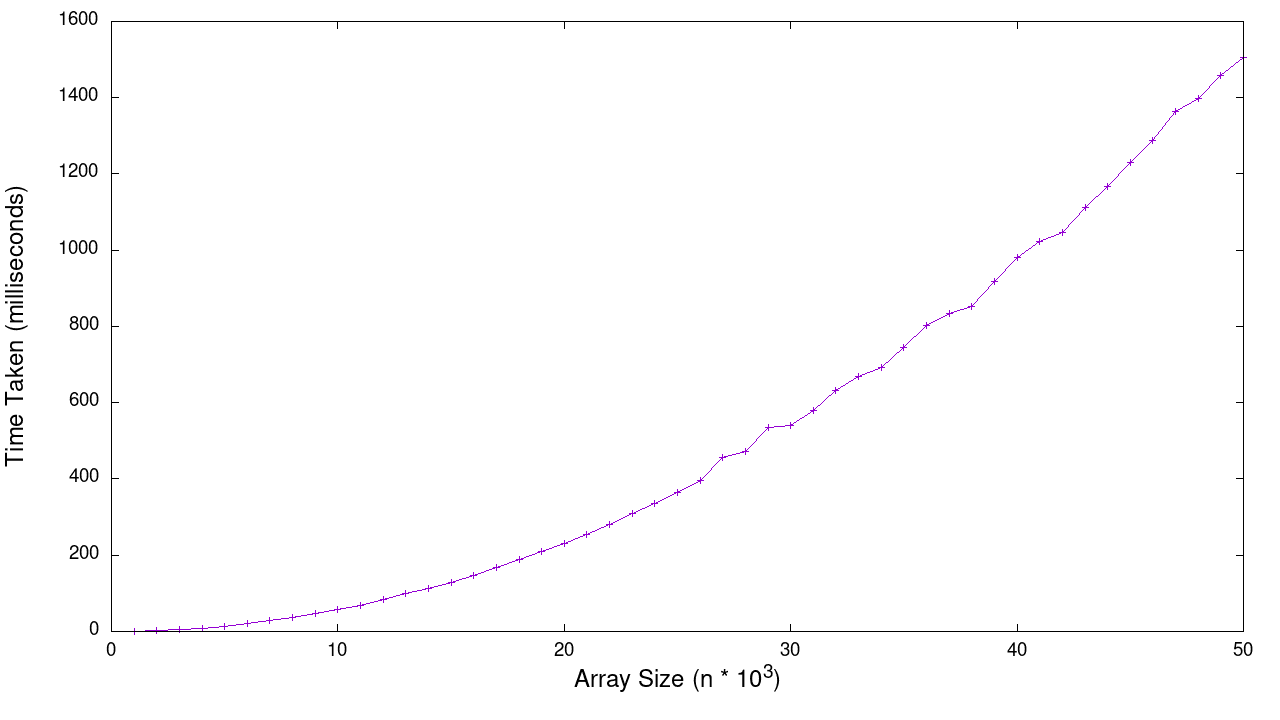
\includegraphics[width=0.8\textwidth]{InsertionSort_plot}
  \caption{Insertion sort, array size plotted against time}
  \label{fig:InsertionSort_plot}
\end{figure}

The outer loop runs $(n - 1)$ iterations in total, while the inner loop has a progressively smaller range
as the sorted subarray grows.
In the worst case, where the array is sorted in reverse order,
the inner loop iterates over the entire length of the sorted subarray for each element,
leading to $(1 + 2 + 3 + \cdots + (n - 1))$ operations.
This gives us a total time complexity of $O(n^2)$.
On the average case, where the order of the array is random, each element will move about halfway through the sorted portion of the array.
The total iterations will grow in the same way as the worst case scenario, quadratically relative to $(n)$,
resulting in a time complexity of $O(n^2)$.
This time complexity can be observed in figure 2.
However, in the best case scenario, where the array is already sorted, the inner loop does not execute any swaps,
it only examines each element.
This leads to the time complexity of the best case scenario to be $O(n)$.

\section*{Merge Sort}

Merge sort works by recursively dividing an array into two halves, sorting each half individually,
and then merging the two sorted halves back together.
The splitting is done by calculating the midpoint index of the array.
Below is the code for the recursive sorting function and mergin process:

\begin{minted}{c}
void sort(int *org, int *aux, int lo, int hi)
{
    if (lo >= hi)
    {
        return;
    }

    int mid = (lo + hi) / 2;

    sort(org, aux, lo, mid);
    sort(org, aux, mid + 1, hi);

    merge(org, aux, lo, mid, hi);
}
\end{minted}

The \texttt{merge} function is responsible for combining the two sorted subarrays into a single sorted array.
It uses an auxiliary storage array to hold copied elements temporarily, ensuring no data is lost while merging:

\begin{minted}{c}
void merge(int *org, int *aux, int lo, int mid, int hi)
{
    for (int k = lo; k <= hi; k++)
    {
        aux[k] = org[k];
    }

    int i = lo;
    int j = mid + 1;

    for (int k = lo; k <= hi; k++)
    {
        if (i > mid)
        {
            org[k] = aux[j++];
        }
        else if (j > hi)
        {
            org[k] = aux[i++];
        }
        else if (aux[i] <= aux[j])
        {
            org[k] = aux[i++];
        }
        else
        {
            org[k] = aux[j++];
        }
    }
}
\end{minted}

\begin{figure}[h!]
    \centering
    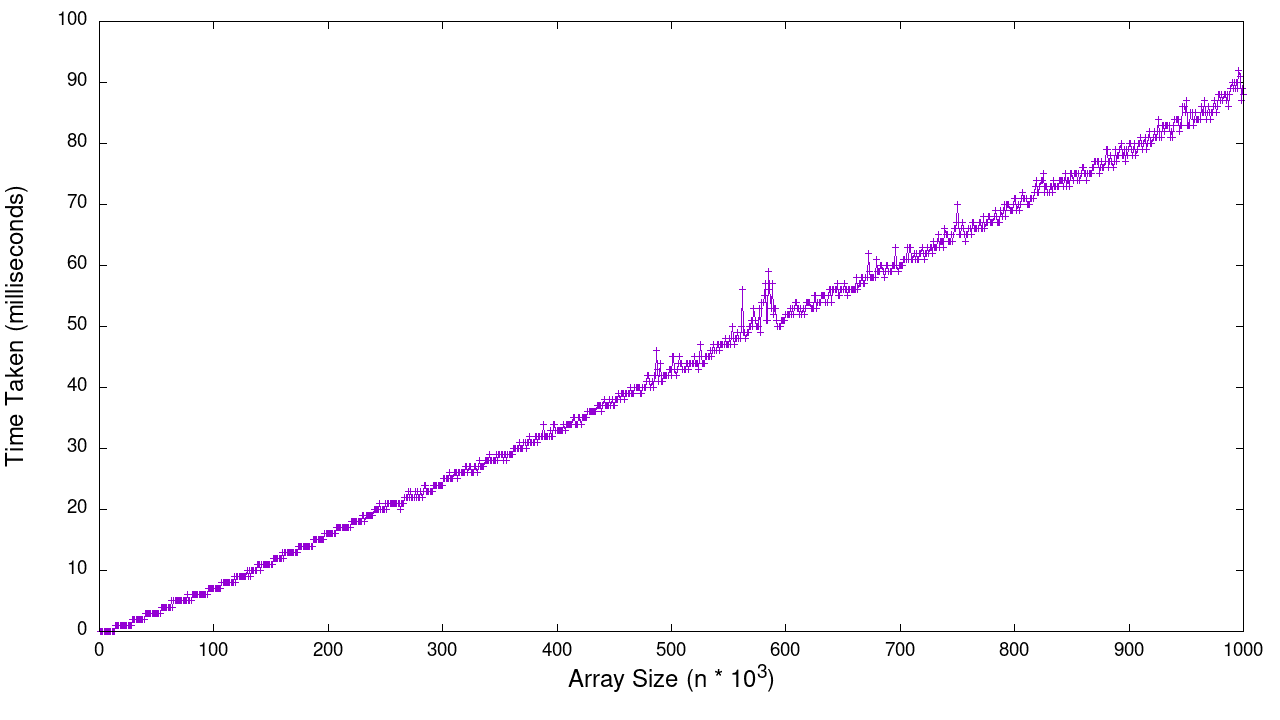
\includegraphics[width=0.8\textwidth]{MergeSort_plot}
    \caption{Merge sort, array size plotted against time}
    \label{fig:MergeSort_plot}
\end{figure}

The merge sort algorithm follows a time complexity of $O(n \log n)$ across all cases.
This performance stems from the fact that the array is split into halves at each step,
resulting in a logarithmic number of divisions, and merging all elements together at each level,
which takes $O(n)$ time.
When looking at figure 3, it could be hard to see that this algorithm would follow $O(n \log n)$ time,
it looks like it is just $O(n)$.
This however, is not fully surprising.
For large $n$, the $n \log n)$-graph looks very similar to that of a linear graph because the linear element scales faster than the logarithmic element.
It can also be noted that the run time of the merge sort algorithm is significantly faster than that of the insertion and selection sort.

\section*{Quick Sort}



\section*{1}

\end{document}
